Tradionnellement, une pizza se coupe en parts égales selon des rayons. Nous décidons de la partager selon des segments issus d'un point fixé \emph{qui n'est pas le centre}.\newline
On considére le disque unité et un point fixé $C$ de coordonnées $(c,0)$ avec $c \in]0,1[$.\newline
La programmation se fera de préférence en SciLab.
\begin{figure}[h]
  \centering
  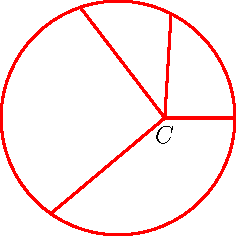
\includegraphics{./Epizza_1_fig.pdf}
  \caption{Un partage inégal.}
  \label{fig:Epizza_1}
\end{figure}
\begin{figure}[h]
  \centering
  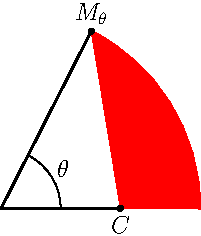
\includegraphics{./Epizza_2_fig.pdf}
  \caption{Angle $\theta$}
  \label{fig:Epizza_2}
\end{figure}
\begin{enumerate}
  \item Exprimer en fonction de $\theta$ et $c$ l'aire de la part repérée par un $\theta$ entre $0$ et $\pi$ comme sur la figure \ref{fig:Epizza_2}.
  \item Pour une valeur de $c$ que vous choisirez, tracer le graphe de cette fonction entre $0$ et $\pi$. Tracer le graphe de sa bijection réciproque. Est-il nécéssaire de savoir calculer cette bijection réciproque pour tracer ce graphe?
  \item Calculer numériquement, le point du cercle qui permet de partager la pizza en quatre parts égales.
  \item Pour un entier $p>2$, implémenter une fonction de $p$ et $c$ qui calcule les points du cercle permettant, en traçant les segements entre ces points et $C$ de partager la pizza en $p$ parts égales. Cette fonction devra aussi tracer le cercle et ces rayons.\newline
\end{enumerate}
